\documentclass[conference]{IEEEtran}
\IEEEoverridecommandlockouts
% The preceding line is only needed to identify funding in the first footnote. If that is unneeded, please comment it out.
%----------------------------------------------------------
\usepackage{cite}
\usepackage[pdftex]{graphicx}
% declare the path(s) where your graphic files are
\graphicspath{images/}
\DeclareGraphicsExtensions{.pdf,.jpeg,.png,.jpg}
\usepackage{amsmath,amssymb,amsfonts}
\usepackage{algorithmic}
\usepackage{graphicx}
\usepackage{textcomp}
\usepackage{array}
%\usepackage[caption=false,font=normalsize,labelfont=sf,textfon =sf]{subfig}
\usepackage{dblfloatfix}
\usepackage{url}
\usepackage{lipsum}
\usepackage{listings}
\usepackage{xcolor}
\def\BibTeX{{\rm B\kern-.05em{\sc i\kern-.025em b}\kern-.08em
    T\kern-.1667em\lower.7ex\hbox{E}\kern-.125emX}}
%----------------------------------------------------------
    \lstset{
        escapeinside={/*@}{@*/},
        language=Python,	
        basicstyle=\fontsize{8.5}{12}\selectfont,
        numbers=left,
        numbersep=2pt,    
        xleftmargin=2pt,
        frame=tb,
        columns=fullflexible,
        showstringspaces=false, 
        tabsize=4,
        keepspaces=true,
        showtabs=false,
        showspaces=false,
        morekeywords={inline,public,class,private,protected,struct},
        captionpos=b,
        lineskip=-0.4em,
        aboveskip=10pt,
        extendedchars=true,
        breaklines=true,
        prebreak = \raisebox{0ex}[0ex][0ex]{\ensuremath{\hookleftarrow}},
        keywordstyle=\color[rgb]{0,0,1},
        commentstyle=\color[rgb]{0.133,0.545,0.133},
        stringstyle=\color[rgb]{0.627,0.126,0.941},
    }
%----------------------------------------------------------

\begin{document}

\title{Comunicação entre dois Arduinos através da conexão serial \\
{\footnotesize \textsuperscript{} Sistemas Embarcados: Prof. Marco Reis - marco.reis@ba.docente.senai.br}
\thanks{Identify applicable funding agency here. If none, delete this.}
}

% \author{\IEEEauthorblockN{Marco Reis, 41650-010\IEEEauthorrefmark{1}}
% \IEEEauthorblockA{\IEEEauthorrefmark{1}Robotics & Autonomous Systems Center,
% Senai Cimatec, Salvador, Brazil}% <-this % stops an unwanted space


\author{\IEEEauthorblockN{Felipe Cauã Ribeiro Pardo Casas}
\IEEEauthorblockA{\textit{Engenharia Elétrica} \\
\textit{Senai Cimatec}\\
Salvador, Brasil \\
felipe.casas@ba.estudante.senai.br}
}

\maketitle

\begin{abstract}
This present has as porpose aims to show the operation of the serial communication between two Arduinos, approaching the concepts of embedded systems seen in the classroom. The objective of the activity is to make the LCD display connected to an Arduino print the value of the distance measured by the ultrasonic sensor connected to another Arduino, through the RX TX serial connection. At the end of the activity, it was possible to understand these concepts, learning in a didactic and playful way the techniques of programming and assembly of electronic circuits, using the Tinkercad simulation platform, corresponding to the proposed objective. Thus, the activity was carried out successfully.

\end{abstract}

\begin{IEEEkeywords}
Embedded System, Arduino, serial communication, Tinkercad.
\end{IEEEkeywords}

\section{Introdução}
Os sistemas embarcados são compostos por uma unidade de processamento, que é um circuito integrado, fixado a um circuito impresso. Os sistemas embarcados podem ser definidos como sistemas que possuem uma capacidade de processamento de informações vinda de um software que está sendo processado internamente nessa unidade. Estes estão cada vez mais baratos e acessíveis, demandam menor consumo de energia e, além de mais compactos, possuem maior poder de processamento. 


Visando compreender os conceitos aplicados em sala de aula a respeito dos sistemas embarcados, e aprendendo na prática de forma lúdica e didática, foi desenvolvido um projeto que envolvem dois sistemas embarcados (dois arduinos), em que um arduino realiza a leitura de uma distância até o objeto e através da conexão serial (RX/TX) o outro arduino imprime esse valor no display que está acoplado nele. 


\section{Objetivo }
O objetivo da atividade é fazer com que um sistema embarcado receba uma String de um outro sistema embarcado e disponibilize esta informação num display, através da conexão serial. 

\section{Referencial teórico}
\subsection{Arduino UNO}
Arduino, visto na figura 1, é uma plataforma de código aberto (hardware e software) criada em 2005 pelo italiano Massimo Banzi (e outros colaboradores) para auxiliar no ensino de eletrônica para estudantes de design e artistas. O objetivo principal foi o de criar uma plataforma de baixo custo, para que os estudantes pudessem desenvolver seus protótipos com o menor custo possível. Outro ponto interessante do projeto, foi a proposta de criar uma plataforma de código aberto, disponível para a comunidade o que ajudou em muito no seu desenvolvimento. O arduino possui 14 pinos de entrada/saída digital (dos quais 6 podem ser usados como saídas PWM) e 6 entradas analógicas.


O componente principal da placa Arduino UNO é o microcontrolador ATMEGA328, um dispositivo de 8 bits da família AVR com arquitetura RISC avançada e com encapsulamento DIP28. Ele conta com 32 KB de Flash, 2 KB de RAM e 1 KB de EEPROM. Pode operar a até 20 MHz, porém na placa Arduino UNO opera em 16 MHz, valor do cristal externo que está conectado aos pinos 9 e 10 do microcontrolador.
\begin{center}
    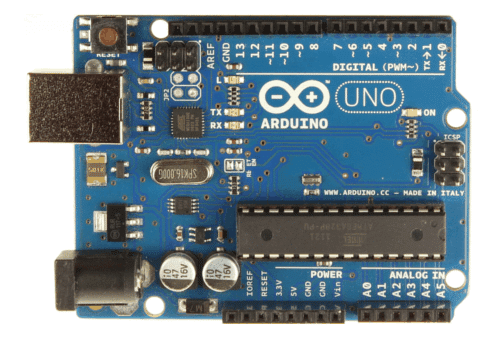
\includegraphics[width=8cm]{Arduino.png}
    Figura 1: Arduino Uno
\end{center}
\subsection{Sensor ultrassônico}
 O modulo ultrassônico HC-SR04, visto na figura 2, possui um transmissor ultrassônico (Trigger), receptor (Echo) e circuito de controle. É necessário dar pulso de disparo, para que ele gere ultrassom de frequência 40 kHz. Este é capaz de ser usado para mensurar distâncias com base na velocidade do som no ar e na diferença de tempo entre emissão e recepção de um sinal ultrassônico. Depois de gerar o ultrassom, ou seja, 8 pulsos de 40 kHz, ele torna o pino Echo alto. O pino Echo permanece alto até que não receba o som de eco de volta. Assim, a largura do pino Echo será o tempo para o som viajar para o objeto e retornar. Uma vez que tenha o tempo, pode-se calcular a distância, pois sabe-se a velocidade do som. O modelo HC-SR04 possui um range para mensurar a distância de 2 cm até 400 cm.
 \begin{center}
    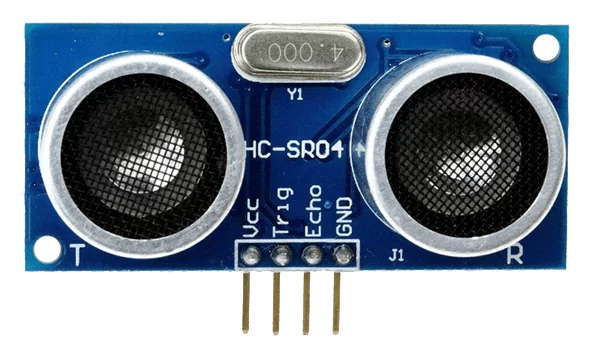
\includegraphics[width=8cm]{Sensor.png}
    Figura 2: Sensor ultrassônico HC-SR04
\end{center}
\subsection{Display LCD}
O Display de Cristal Líquido (LCD), visto na figura 3, é amplamente utilizado em várias aplicações eletrônicas. É comumente usado em vários sistemas para mostrar diferentes status e parâmetros. LCD16x2 tem 2 linhas com 16 caracteres em cada linha. Cada caractere é composto por uma matriz de pixels de 5x8.

O display LCD pode operar em dois modos: 8 bits ou 4 bits, no modo oito bits utilizam-se os pinos numerados de DB0 a DB7, o qual estão dispostos do menos significativo ao mais significativo, ou seja,  os oito bits correspondentes ao modo de operação são os oito pinos físicos do hardware que funcionam em conjunto com os pinos de controle. Na configuração 4 bits apenas quatro pinos GPIO estão conectados ao pino de dados LCD (D4-D7), o que ajuda a economizar pinos GPIO. Por padrão, o LCD16x2 está no modo de 8 bits. Para usar o LCD16x2 no modo de 4 bits, é necessário enviar alguns comandos para inicialização e configuração do LCD.

 \begin{center}
    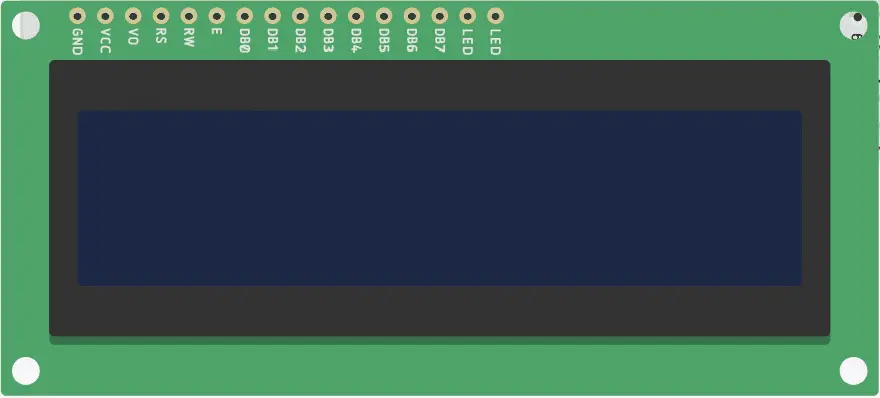
\includegraphics[width=8cm]{LCD.png}
    Figura 3: Display LCD 16x2
\end{center}
\subsection{Comunicação Serial UART}
UART (Universal Asynchronous Receiver Transmitter) é um protocolo de comunicação serial usado para transmitir/receber dados serialmente em uma taxa de transmissão específica. Com a ajuda do UART, pode-se enviar/receber dados para um computador ou outros dispositivos. Operação assíncrona significa que um processo opera independentemente de outros processos, cada caractere (byte de dados) é colocado entre os bits de início e fim. A taxa de transferência de dados na comunicação de dados serial é indicada em bits por segundo. O Arduino se comunica com dispositivos seriais através dos pinos digitais 0 (RX) e 1 (TX). Para os bits serem transmitidos e recebidos, o transmissor e o receptor devem estar configurados com o mesmo valor de baudrate, dado em bits por segundo, que é a taxa de transmissão de dados entre um dispositivo a outro.
\section{Materiais}
A montagem do circuito, simulação e a programação foram feitas no Software Tinkercad com auxílio do Arduino IDE.

Os materiais utilizados na elaboração do projeto foram:

 \begin{itemize}
     \item 1 Protoboard; 
     \item 2 Arduinos UNO;
     \item 3 Leds (Verde, amarelo e vermelho);
     \item 4 Resistores de $ 220\Omega $;
     \item 1 Resistor de $ 1K\Omega $;
     \item 1 Display LCD 16X2;
     \item 1 Sensor ultrassônico HC-SR04;
 \end{itemize}

\section{Procedimentos experimentais }
\subsection{Construção}
Inicialmente foram adicionados os componentes que seriam utilizados no projeto. Foram separados dois arduinos, em que um terá a função de emitir os dados e o outro irá receber estes dados. Em seguida foi montado o circuito, conectando componentes nas portas digitais dos arduinos e na alimentação, com auxílio da protoboard, como visto na figura 4. O modulo HC-SR04 e os leds foram conectados ao Arduino principal (Emissor) e o LCD foi conectado ao Arduino secundário (receptor). Para a comunicação do Display LCD com o Arduino foram utilizando apenas 4 das 8 portas de dados do display conectadas nas portas digitais. Prontamente foi feita a comunicação serial, conectando a porta TX do arduino emissor na porta RX do arduino receptor, e a porta RX do arduino emissor na porta TX do arduino receptor. 


\begin{center}
    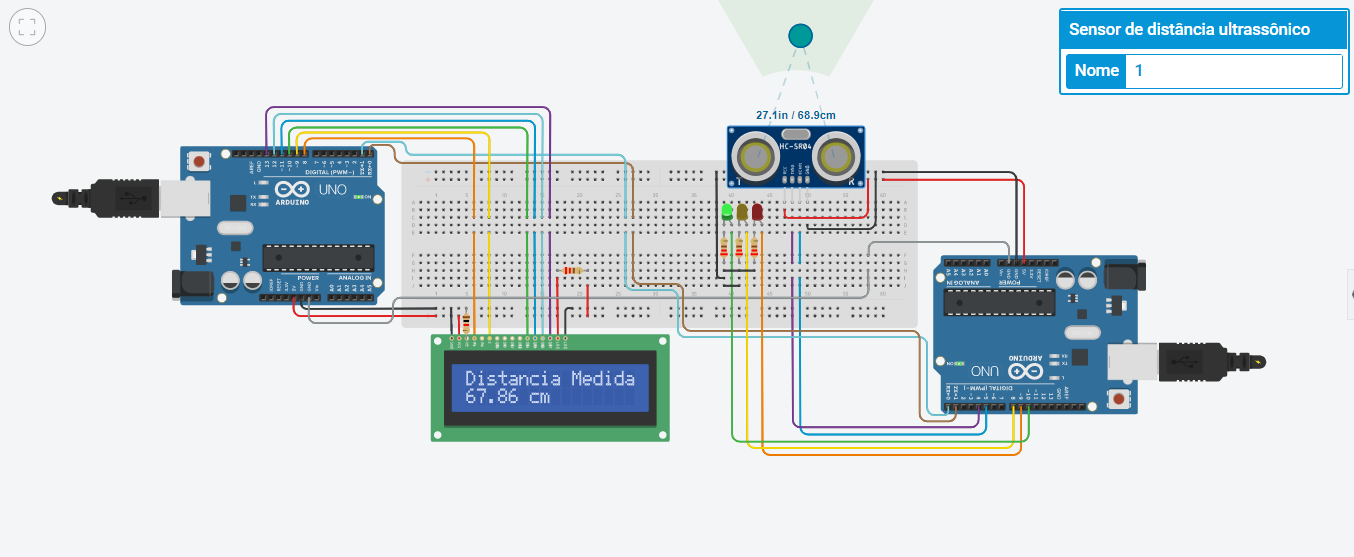
\includegraphics[width=9cm]{Esquematico.png}
    Figura 4: Esquemático do circuito
\end{center}

\subsection{Programação}
Partindo para a programação, primeiramente foram declaradas as portas digitais utilizadas e as variáveis, adicionadas as bibliotecas do display LCD e da função String, e por fim, foi definida a taxa de transmissão da comunicação serial (9600 bits por segundo). No Arduino principal foram feitas as condições para os leds acenderem em determinada região, estas distâncias podem ser vistas na tabela 1. Por fim, foi colocada a sintaxe “Serial.println”, em que vai imprimir dados da leitura do sensor na comunicação serial como texto ASCII legível seguido por um caractere do retorno da transmissão e um caractere de nova linha (barra "n").

\begin{center}
   Tabela 1- Regiões de acionamento para cada led
\end{center}
\begin{tabular}{c|c|c|c}\hline
\textbf{Leds} & \textbf{Verde} & \textbf{Amarelo} & \textbf{Vermelho}  \\\hline
   \textbf{Distancia mínima}  & 0 cm & 110 cm & 220 cm \\
     \textbf{Distancia máxima} & 110 cm & 220cm & 330 cm \\ 
\end{tabular}
\begin{center}
  Fonte: Própria
\end{center}

 No Arduino secundário foi declarada uma variável "Distância" do tipo String. No void loop foi feita uma condição para verificar se há alguma informação vinda da comunicação serial, ou seja, do arduino principal, se tiver, ele vai lê os caracteres do buffer serial em uma String, em seguida vai esperar a transmissão de dados seriais enviados terminar. Prontamente, estes dados serão enviados para o display LCD para que este imprima esses valores na tela. O display vai imprimir o texto "Distância medida", o valor da distância e a unidade de medida, que no caso é o centímetro (cm), como visto na figura 5.
\begin{center}
    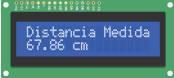
\includegraphics[width=8cm]{LCD-on.png}
    Figura 5: Display LCD ligado
\end{center}

\subsection{Criação do Artigo}
Com a atividade finalizada foi feita a confecção do artigo utilizando o software Visual Studio Code e a linguagem Latex, abordando tudo que foi feito, observado e compreendido ao decorrer da atividade.
\section{resultados e discussão}
Após testes e simulações com o sensor ultrassônico, constatou-se que o mesmo teria uma grande margem de erro na leitura da distância, isso pode se dar, devido a própria simulação do tinkercad, pois não se sabe a velocidade do som na simulação, já que a velocidade do som está diretamente relacionada com o cálculo da distância. 


Com o circuito montado e as programações feitas, ao realizar as simulações foi possível notar que ao diminuir o valor do delay no void loop não havia a comunicação de informações do Arduino principal para o secundário, sendo um delay de 5 segundos para imprimir um novo valor do sensor no display LCD. 


\section{Conclusão}
 Apesar de haver uma margem de erro na leitura do sensor ultrassônico e um significativo delay para atualizar os valores no painel LCD, ao final foi possível corresponder ao objetivo proposto, sendo feita a comunicação serial entre dois Arduinos, compreendendo os conceitos do sistema embarcado visto em sala de aula. Os acionamentos dos leds para determinadas regiões funcionou corretamente. Desse modo, a atividade foi realizada com êxito. 

\section *{Referências}
     [1] Arduino. Arduino, 2022. Disponível em: www.arduino.cc. Acesso em: 18 de maio de 2022;
    
     [2] Ciriaco, Douglas. O que é Arduino?. Canal Tech,
2015. Disponível em: https://canaltech.com.br/hardware/o-que-e-arduino/. Acesso em: 18 de maio de 2022.

     [3] Equipe FILIPEFLOP, 2022. Como utilizar o Display LCD (16x2) no Arduino?
Disponível em: https://www.filipeflop.com/blog/como-utilizar-o-display-lcd-16x2/. Acesso em: 18 de maio de 2022.
\end{document}